\documentclass{article}
\usepackage[utf8]{inputenc}
\usepackage[margin=1in]{geometry}

\title{348 - Homework 12}
\author{Victor Zhang}
\date{April 22, 2021}

\usepackage[utf8]{inputenc}
\usepackage{amsmath}
\usepackage{amsfonts}
\usepackage{natbib}
\usepackage{graphicx}
% \usepackage{changepage}
\usepackage{amssymb}
\usepackage{xfrac}
% \usepackage{bm}
% \usepackage{empheq}
\usepackage{subcaption}
\usepackage{dirtytalk}
\usepackage{hhline}
\usepackage{hyperref}

\hypersetup{
    colorlinks=true,
    linkcolor=blue,
    filecolor=magenta,      
    urlcolor=cyan,
}

\urlstyle{same}

\newcommand{\contra}{\raisebox{\depth}{\#}}

\newenvironment{myindentpar}[1]
  {\begin{list}{}
          {\setlength{\leftmargin}{#1}}
          \item[]
  }
  {\end{list}}

\pagestyle{empty}

\begin{document}

\maketitle
% \begin{center}
% {\huge Econ 482 \hspace{0.5cm} HW 3}\
% {\Large \textbf{Victor Zhang}}\
% {\Large February 18, 2020}
% \end{center}

\section*{6.1.a}
$m = (-5-2)/(3-0) = -\frac{7}{3}$. $x = m^2 - x_1 - x_2 = \frac{49}{9} - 3 = \frac{22}{9}$. $y = -(-\frac{7}{3}\frac{22}{9}+2) = \frac{100}{27}$. $P + Q = (\frac{22}{9},\frac{100}{27})$.

\section*{6.1.b}
$m = \frac{3x^2-2}{2\cdot2} = -\frac{1}{2}$. $x = m^2 - x_1 - x_1 = \frac{1}{4}$. $y = -(-\frac{1}{2}\frac{1}{4}+2) = -\frac{15}{8}$. $P + P = (\frac{1}{4},-\frac{15}{8})$.\\
$m = \frac{25}{-10} = -\frac{5}{2}$. $x = \frac{25}{4} - 6 = \frac{1}{4}$. $y = -(-\frac{5}{2}\frac{1}{4} + \frac{5}{2}) = -\frac{15}{8}$. $Q + Q = (\frac{1}{4}, -\frac{15}{8})$.

\section*{6.1.c}
$P + P + P = (\frac{1}{4},-\frac{15}{8}) + P$. $m = -\frac{31}{2}$. $x = 240$. $y = 3718$. $P + P + P = (240,3718)$.\\
$Q + Q + Q = (\frac{1}{4},-\frac{15}{8}) + Q$. $m = -\frac{25}{22}$. $x = -\frac{237}{121}$. $y = -\frac{845}{1331}$. $Q + Q + Q = (-\frac{237}{121},-\frac{845}{1331})$.

\section*{6.3}
First let us note $e_1 + e_2 + e_3 = 0$, so write $e_3 = - e_1 - e_2$. Then
$$(X - e_1)(X - e_2)(X + e_1 + e_2) = X^3 - (e_1^2 + e_1e_2 + e_2^2)X + e_1e_2(e_1+e_2)$$
Then we may write
$$4A^3 + 27B^2 = -4 e_1^6 - 12 e_1^5 e_2 + 3 e_1^4 e_2^2 + 26 e_1^3 e_2^3 + 3 e_1^2 e_2^4 - 12 e_1 e_2^5 - 4 e_2^6$$
which factors as
$$-(e_1-e_2)^2(e_1+e_1+e_2)^2(e_2+e_1+e_2)^2 = -(e_1-e_2)^2(e_1-e_3)^2(e_2-e_3)^2$$
This is identically 0 iff at least two of $e_1,e_2,e_3$ are equal $\Box$

\section*{6.4}
\begin{figure*}[h!]
\begin{subfigure}[h]{0.3\linewidth}
  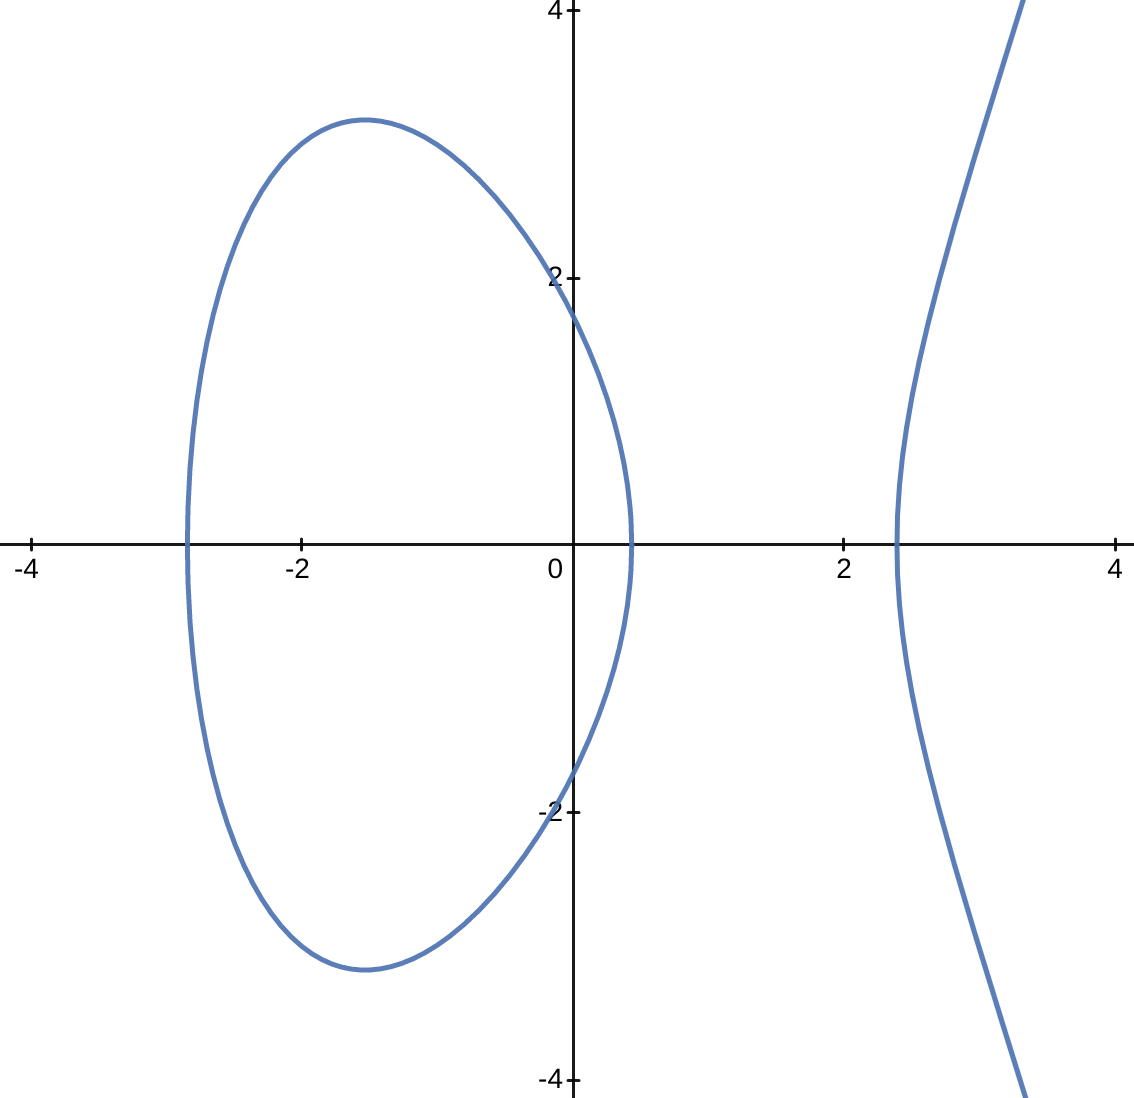
\includegraphics[width=\linewidth]{img/hw_12_1.png}
  \caption{$E: Y^2 = X^3 - 7X + 3$}
\end{subfigure}
\hfill
\begin{subfigure}[h]{0.3\linewidth}
  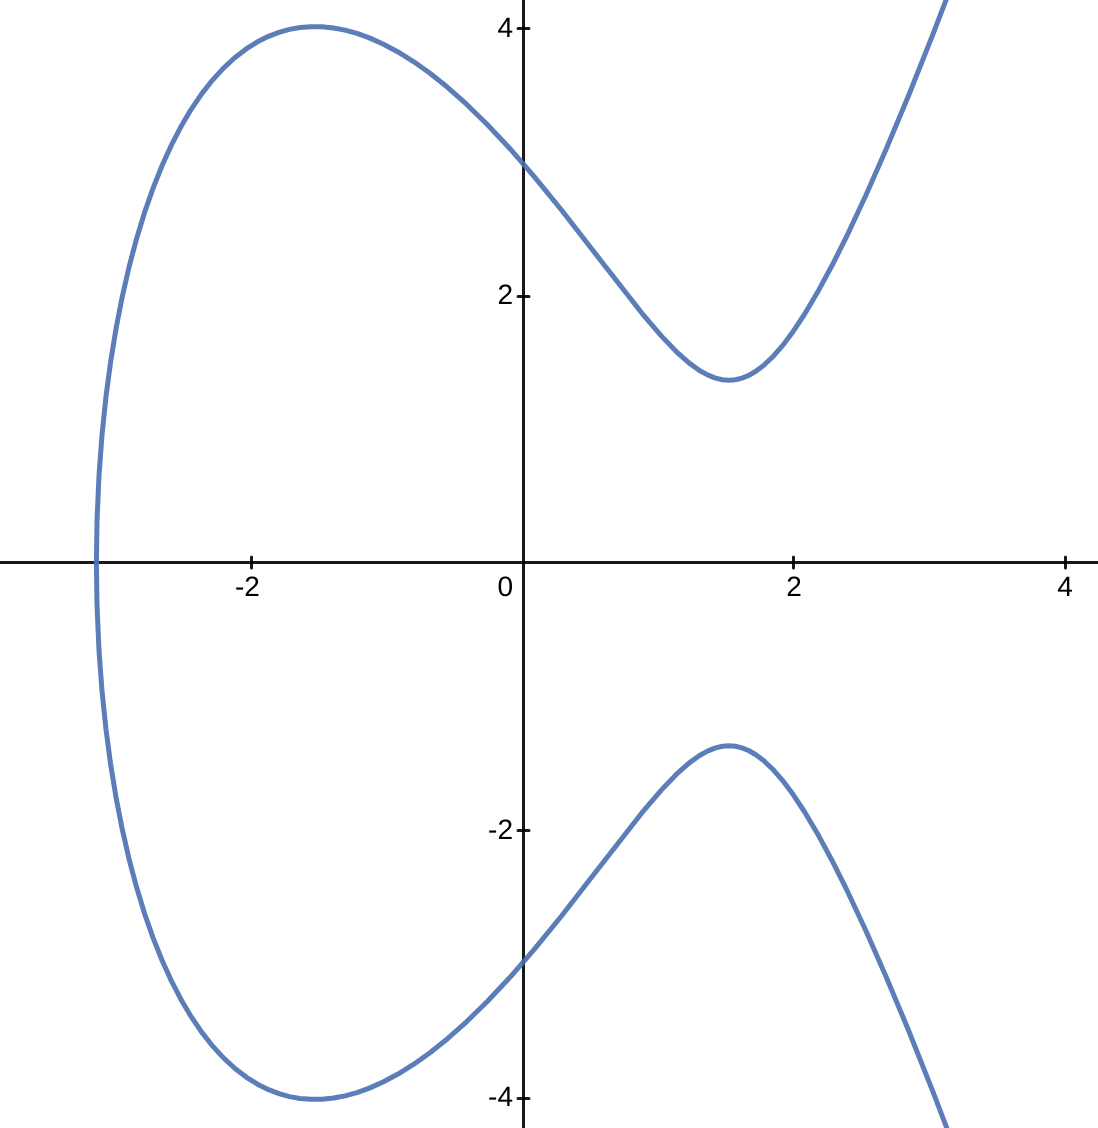
\includegraphics[width=\linewidth]{img/hw_12_2.png}
  \caption{$E: Y^2 = X^3 - 7X + 9$}
\end{subfigure}
\hfill
\begin{subfigure}[h]{0.3\linewidth}
  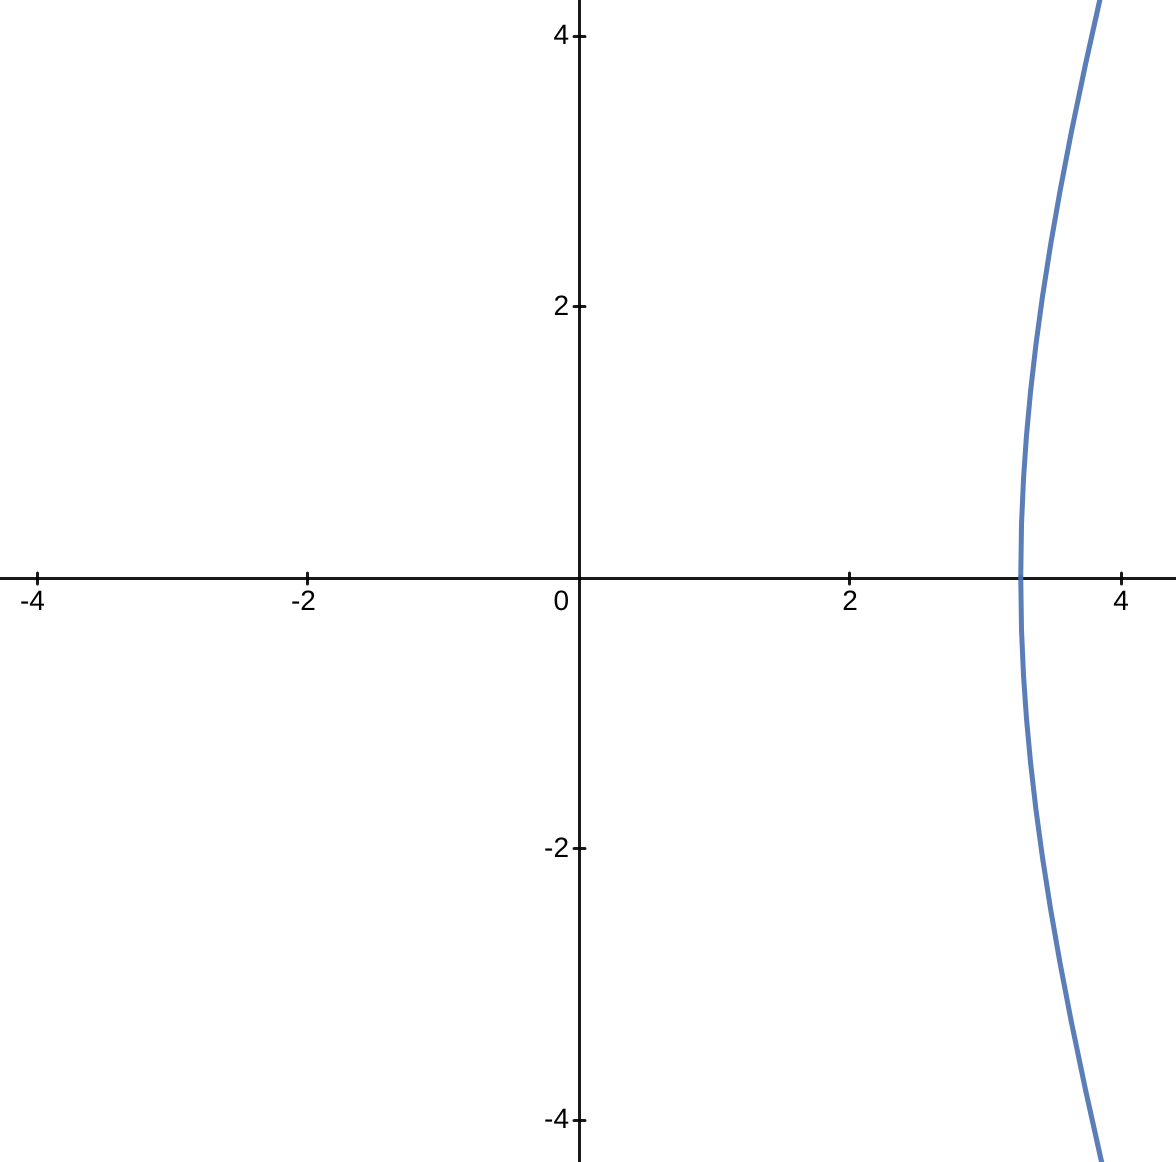
\includegraphics[width=\linewidth]{img/hw_12_3.png}
  \caption{$E: Y^2 = X^3 - 7X + -12$}
\end{subfigure}%

\hfil
\begin{subfigure}[h]{0.3\linewidth}
  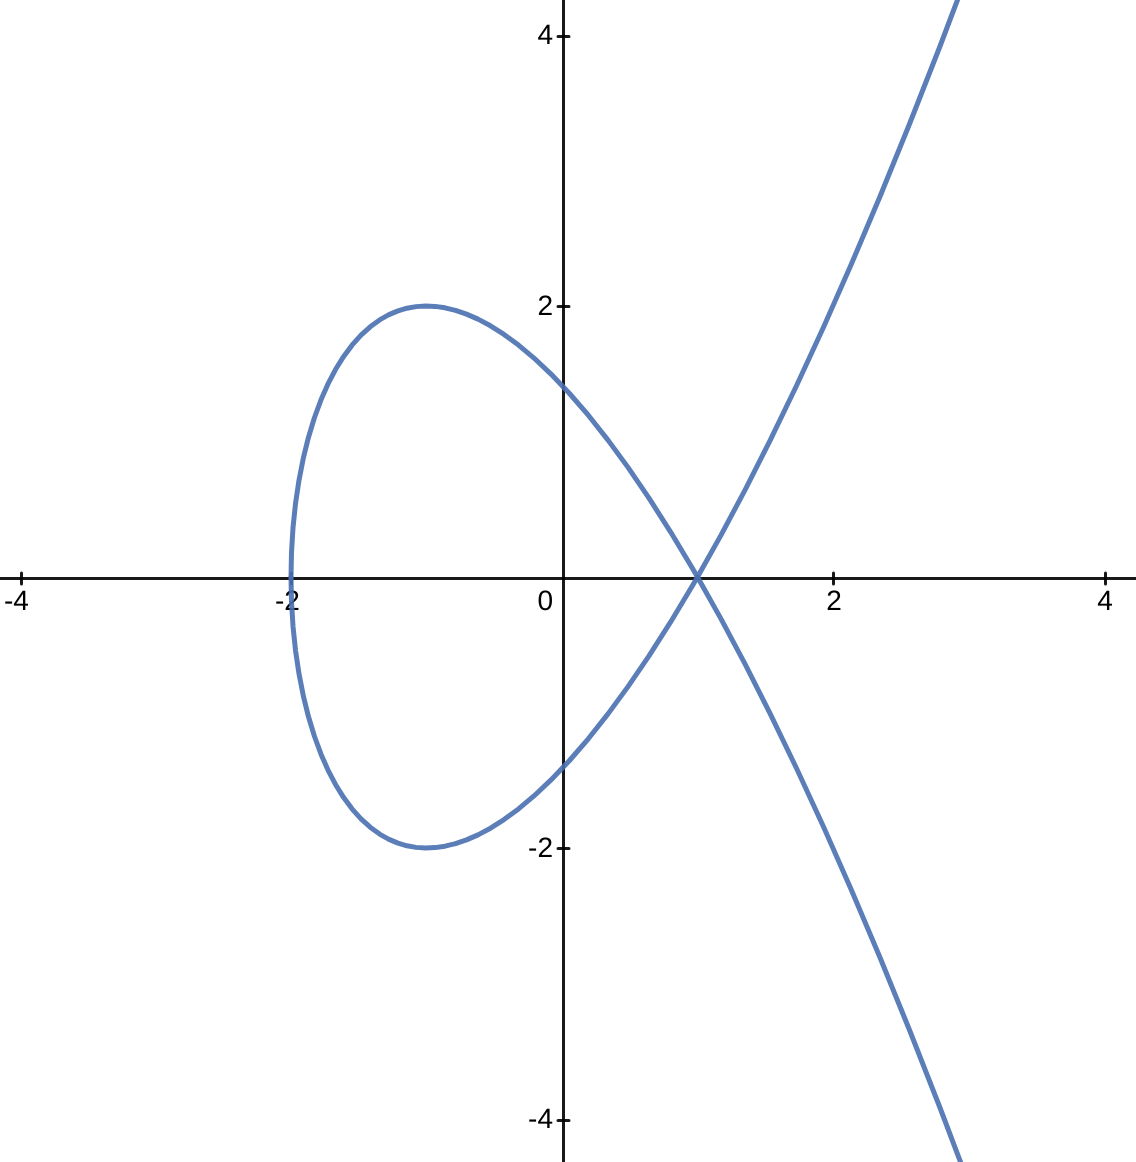
\includegraphics[width=\linewidth]{img/hw_12_4.png}
  \caption{$E: Y^2 = X^3 - 3X - 2$}
\end{subfigure}
\hfil
\begin{subfigure}[h]{0.3\linewidth}
  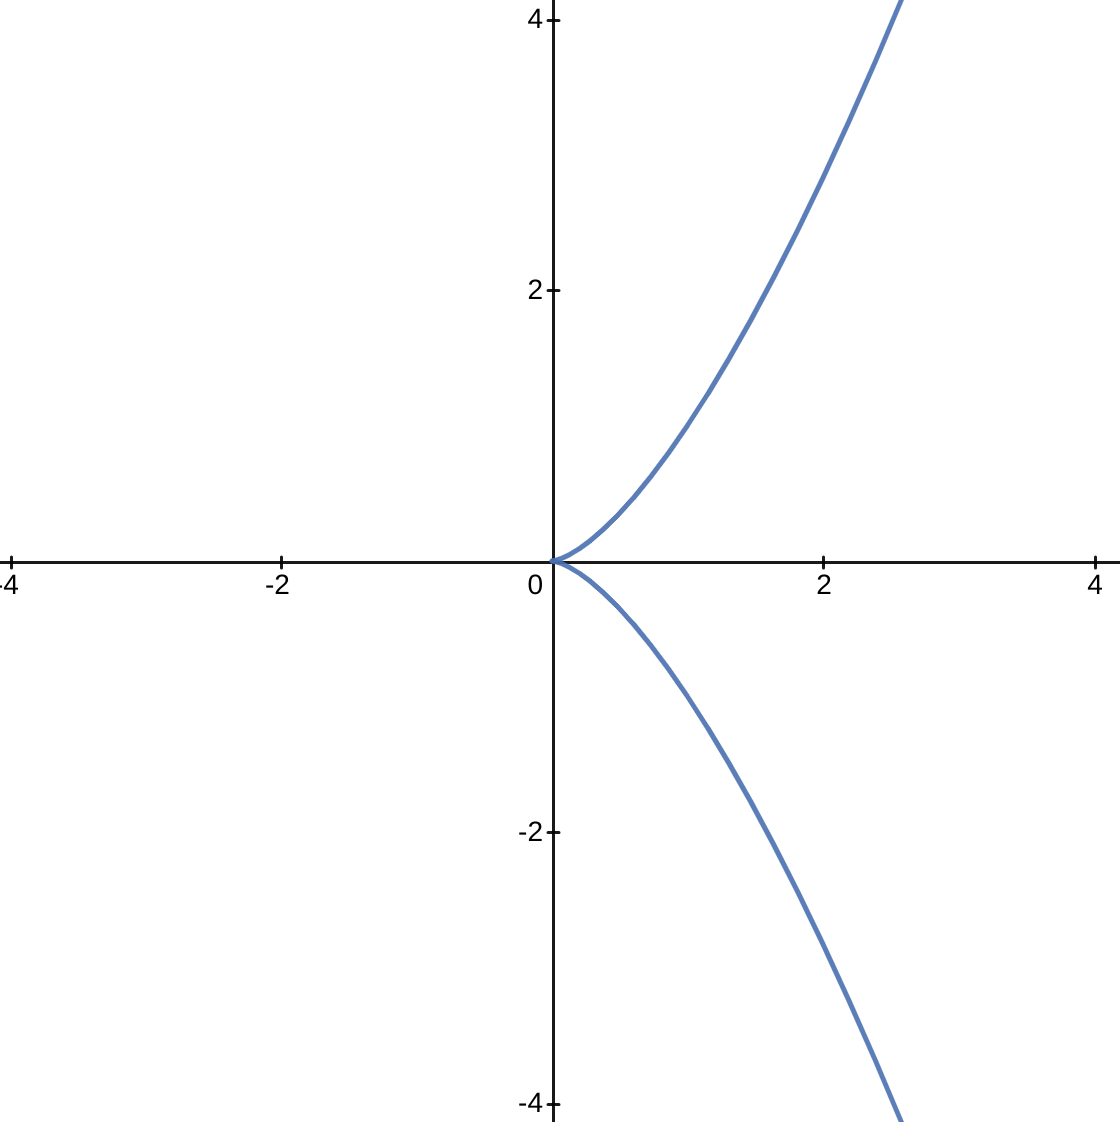
\includegraphics[width=\linewidth]{img/hw_12_5.png}
  \caption{$E: Y^2 = X^3$}
\end{subfigure}
\caption{Plots for 6.4}
\label{fig:fig1}
\end{figure*}

From figure \ref{fig:fig1}, we see the curves d,e have sharp turns in the graph. That is, they are not differentiable at certain points so we cannot double these \say{singular} points.

\section*{6.5.a}
We first note the quadratic residues mod 7 are 0, 1, 2, 4. By bruteforce listing, we get $O$, (0,3), (0,4), (2,3), (2,4), (4,1), (4,6), (5,3), (5,4).

\section*{6.5.c}
The quadratic residues mod 11 are 0, 1, 3, 4, 5, 9. We list the points as $O$, (0,4), (0,7), (3, 0), (6,5), (6,6), (9,0), (10,0).

\section*{6.6.a}
The points of $E(\mathbb{F}_5)$ are $\{O, (1,2), (1,3), (4,0)\}$. We write the table as

\begin{tabular}{|c||c|c|c|c|}
\hline
+ & $O$ & (1,2) & (1,3) & (4,0)\\
\hhline{|=#=|=|=|=|}
$O$ & $O$ & (1,2) & (1,3) & (4,0)\\
\hline
(1,2) & (1,2) & (4,0) & $O$ & (1,3)\\
\hline
(1,3) & (1,3) & $O$ & (4,0) & (1,2)\\
\hline
(4,0) & (4,0) & (1,3) & (1,2) & $O$\\
\hline
\end{tabular}

\section*{6.8}
We bruteforce compute the multiples of $P$ as $2P = (3,4)$, $3P = (2,4)$, $4P = (0,4)$, $5P = (0,1)$. So $Q = 5P$.

\section*{6.11.a}
We compute the tuple $(n,P^i, Q)$ at each step $i$:\\
(9,(30,8),(24,14))\\
(4,(24,69),(30,75))\\
(2,(30,75),(30,75))\\
(1,(24,14),(30,75))\\
(0,(30,8),(24,69))\\
So $19 \cdot (24,14) = (24,69)$.

\section*{6.14.a}
Using a calculator, we get that Bob sends $1943P = (1432,667)$.

\section*{6.14.b}
Their secret shared point is $n_BQ_A = (2424,911)$. The secret shared value is the $x$-coordinate of this point, or 2424.

\end{document}

% List of tex snippets:
%   - tex-header (this)
%   - R      --> \mathbb{R}
%   - Z      --> \mathbb{Z}
%   - B      --> \mathcal{B}
%   - E      --> \mathcal{E}
%   - M      --> \mathcal{M}
%   - m      --> \mathfrak{m}({#1})
%   - normlp --> \norm{{#1}}_{L^{{#2}}}
